\begin{figure}[htbp]
			\centering
			\resizebox{\textwidth}{!}{%
				\begin{tikzpicture}[
					trave/.style={line width=1.8pt, line cap=round, line join=round, black},
					terra/.style={line width=0.8pt, black},
					diag/.style={line width=0.90pt, black},
					nodoV/.style={circle, fill=white, draw=black,
						inner sep=0pt, minimum size=5.0pt, line width=0.80pt},
					segno/.style={circle, draw=black, fill=white, inner sep=0pt,
						minimum size=8pt, font=\tiny, line width=0.55pt},
					etlab/.style={circle, draw=black, line width=0.6pt,
						fill=white, inner sep=2pt, font=\small},
					lab/.style={font=\small},
					]
					
					\def\L{1.80}
					\def\SEP{5.80}
					\def\dNo{0.55}
					\def\dTo{0.30}
					\def\dMo{0.75}
					\def\ext{0.09}  % estensione sopra traverso per visibilità chiusura in D
					
					\def\portale{\draw[trave](0,0)--(0,\L)--(2*\L,\L)--(2*\L,0);}
					\def\cernieraA{%
						\draw[terra](0,0)--(-0.24,-0.40)--(0.24,-0.40)--cycle;
						\draw[terra](-0.34,-0.40)--(0.34,-0.40);
						\foreach \x in {-0.28,-0.16,-0.04,0.08,0.20,0.30}
						\draw[very thin](\x,-0.40)--++(-0.08,-0.11);
						\node[nodoV]at(0,0){};}
					\def\cernieraB{%
						\draw[terra](2*\L,0)--(2*\L-0.24,-0.40)--(2*\L+0.24,-0.40)--cycle;
						\draw[terra]({2*\L-0.34},-0.40)--({2*\L+0.34},-0.40);
						\foreach \x in {-0.28,-0.16,-0.04,0.08,0.20,0.30}
						\draw[very thin]({2*\L+\x},-0.40)--++(-0.08,-0.11);
						\node[nodoV]at(2*\L,0){};}
					
					%%═══ PANNELLO (a) — N₁ ═════════════════════════════════════════════════
					\begin{scope}[xshift=0cm]
						\fill[gray!20](-\dNo,0)--(0,0)--(0,\L)--(-\dNo,\L)--cycle;
						\foreach \y in {0.15,0.30,...,1.75}{\draw[gray!50,very thin](-\dNo,\y)--(0,\y);}
						\draw[diag](-\dNo,0)--(-\dNo,\L);
						\draw[diag](-\dNo,0)--(0,0);
						\draw[diag](-\dNo,\L)--(0,\L);
						\fill[gray!20]({2*\L-\dNo},0)--(2*\L,0)--(2*\L,\L)--({2*\L-\dNo},\L)--cycle;
						\foreach \y in {0.15,0.30,...,1.75}{\draw[gray!50,very thin]({2*\L-\dNo},\y)--(2*\L,\y);}
						\draw[diag]({2*\L-\dNo},0)--({2*\L-\dNo},\L);
						\draw[diag]({2*\L-\dNo},0)--(2*\L,0);
						\draw[diag]({2*\L-\dNo},\L)--(2*\L,\L);
						\fill[gray!20](0,\L)--(2*\L,\L)--(2*\L,{\L+\dNo})--(0,{\L+\dNo})--cycle;
						\foreach \x in {0.35,0.70,...,3.50}{\draw[gray!50,very thin](\x,\L)--(\x,{\L+\dNo});}
						\draw[diag](0,{\L+\dNo})--(2*\L,{\L+\dNo});
						\draw[diag](0,\L)--(0,{\L+\dNo});
						\draw[diag](2*\L,\L)--(2*\L,{\L+\dNo});
						\portale \cernieraA \cernieraB
						\node[nodoV]at(\L,\L){};
						\node[segno]at({-\dNo/2},{\L*0.50}){$-$};
						\node[segno]at({2*\L-\dNo/2},{\L*0.50}){$+$};
						\node[segno]at({0.5*\L},{\L+\dNo/2}){$+$};
						\node[segno]at({1.5*\L},{\L+\dNo/2}){$+$};
						\node[left=0.04,lab]at(-\dNo,{\L*0.50}){$\tfrac{1}{2\ell}$};
						\node[left=0.04,lab]at({2*\L-\dNo},{\L*0.50}){$\tfrac{1}{2\ell}$};
						\node[above=0.04,lab]at(\L,{\L+\dNo}){$\tfrac{1}{2\ell}$};
						\node[right,lab]at(0,0){$A$};
						\node[right,lab]at(2*\L,0){$B$};
						\node[above left,lab]at(0,\L){$C$};
						\node[above right,lab]at(2*\L,\L){$D$};
						\node[below,lab]at(\L,\L){$M$};
						\node[etlab]at(\L,{0}){$N_1$};
					\end{scope}
					
					%%═══ PANNELLO (b) — T₁ ═════════════════════════════════════════════════
					\begin{scope}[xshift=\SEP cm]
						\fill[gray!20](0,0)--(\dTo,0)--(\dTo,\L)--(0,\L)--cycle;
						\foreach \y in {0.15,0.30,...,1.75}{\draw[gray!50,very thin](0,\y)--(\dTo,\y);}
						\draw[diag](\dTo,0)--(\dTo,\L);
						\draw[diag](0,0)--(\dTo,0);
						\draw[diag](0,\L)--(\dTo,\L);
						\fill[gray!20]({2*\L-\dTo},0)--(2*\L,0)--(2*\L,\L)--({2*\L-\dTo},\L)--cycle;
						\foreach \y in {0.15,0.30,...,1.75}{\draw[gray!50,very thin]({2*\L-\dTo},\y)--(2*\L,\y);}
						\draw[diag]({2*\L-\dTo},0)--({2*\L-\dTo},\L);
						\draw[diag]({2*\L-\dTo},0)--(2*\L,0);
						\draw[diag]({2*\L-\dTo},\L)--(2*\L,\L);
						\fill[gray!20](0,\L)--(2*\L,\L)--(2*\L,{\L+\dTo})--(0,{\L+\dTo})--cycle;
						\foreach \x in {0.35,0.70,...,3.50}{\draw[gray!50,very thin](\x,\L)--(\x,{\L+\dTo});}
						\draw[diag](0,{\L+\dTo})--(2*\L,{\L+\dTo});
						\draw[diag](0,\L)--(0,{\L+\dTo});
						\draw[diag](2*\L,\L)--(2*\L,{\L+\dTo});
						\portale \cernieraA \cernieraB
						\node[nodoV]at(\L,\L){};
						\node[segno]at(\dTo/2,{\L*0.50}){$+$};
						\node[segno]at({2*\L-\dTo/2},{\L*0.50}){$-$};
						\node[segno]at({0.5*\L},{\L+\dTo/2}){$+$};
						\node[segno]at({1.5*\L},{\L+\dTo/2}){$+$};
						\node[right=0.04,lab]at(\dTo,{\L*0.50}){$\tfrac{1}{2\ell}$};
						\node[left=0.04,lab]at({2*\L-\dTo},{\L*0.50}){$\tfrac{1}{2\ell}$};
						\node[above=0.04,lab]at(\L,{\L+\dTo}){$\tfrac{1}{2\ell}$};
						\node[left,lab]at(0,0){$A$};
						\node[right,lab]at(2*\L,0){$B$};
						\node[above left,lab]at(0,\L){$C$};
						\node[above right,lab]at(2*\L,\L){$D$};
						\node[below,lab]at(\L,\L){$M$};
						\node[etlab]at(\L,{0}){$T_1$};
					\end{scope}
					
					%%═══ PANNELLO (c) — M₁ ═════════════════════════════════════════════════
					\begin{scope}[xshift={2*\SEP cm}]
						%% M col. sin. (negativo, trapezio a sinistra: dMo in A, dMo/2 in C)
						\fill[gray!20](0,0)--(-\dMo,0)--(-\dMo/2,\L)--(0,\L)--cycle;
						\begin{scope}
							\clip(0,0)--(-\dMo,0)--(-\dMo/2,\L)--(0,\L)--cycle;
							\foreach \y in {0.15,0.30,...,1.75}
							{\draw[gray!50,very thin]({-\dMo-0.1},\y)--(0.1,\y);}
						\end{scope}
						\draw[diag](-\dMo,0)--(-\dMo/2,\L);
						\draw[diag](-\dMo,0)--(0,0);
						\draw[diag](-\dMo/2,\L)--(0,\L);
						%% M col. des. (positivo, triangolo a sinistra di BD — fibra tesa interna)
						\fill[gray!20](2*\L,0)--(2*\L,\L)--({2*\L-\dMo/2},\L)--cycle;
						\begin{scope}
							\clip(2*\L,0)--(2*\L,\L)--({2*\L-\dMo/2},\L)--cycle;
							\foreach \y in {0.15,0.30,...,1.75}
							{\draw[gray!50,very thin]({2*\L-\dMo/2-0.1},\y)--(2*\L+0.1,\y);}
						\end{scope}
						\draw[diag](2*\L,0)--({2*\L-\dMo/2},\L);   % faccia inclinata
						\draw[diag]({2*\L-\dMo/2},\L)--(2*\L,\L);   % chiusura in D (coperta dalla trave)
						%% M traverso metà sin. (negativo, triangolo sopra: dMo/2 in C, 0 in M)
						\fill[gray!20](0,\L)--(0,{\L+\dMo/2})--(\L,\L)--cycle;
						\begin{scope}
							\clip(0,\L)--(0,{\L+\dMo/2})--(\L,\L)--cycle;
							\foreach \x in {0.25,0.50,...,1.75}
							{\draw[gray!50,very thin](\x,{\L-0.1})--(\x,{\L+\dMo/2+0.1});}
						\end{scope}
						\draw[diag](0,{\L+\dMo/2})--(\L,\L);
						\draw[diag](0,\L)--(0,{\L+\dMo/2});
						%% M traverso metà des. (positivo, triangolo sotto: 0 in M, dMo/2 in D)
						\fill[gray!20](\L,\L)--(2*\L,{\L-\dMo/2})--(2*\L,\L)--cycle;
						\begin{scope}
							\clip(\L,\L)--(2*\L,{\L-\dMo/2})--(2*\L,\L)--cycle;
							\foreach \x in {1.90,2.15,...,3.55}
							{\draw[gray!50,very thin](\x,{\L-\dMo/2-0.1})--(\x,{\L+0.1});}
						\end{scope}
						\draw[diag](\L,\L)--(2*\L,{\L-\dMo/2});
						\draw[diag](2*\L,{\L-\dMo/2})--(2*\L,\L);
						%% Archetto di continuità in C (col. sin. → trav. sin.)
						\draw[diag](-\dMo/2,\L) arc(180:90:\dMo/2);
						%% Archetto di continuità in D (trav. des. → col. des.)
						\draw[diag](2*\L,{\L-\dMo/2}) arc(270:180:\dMo/2);
						%% Struttura
						\portale \cernieraA \cernieraB
						\node[nodoV]at(\L,\L){};
						%% Valori
						\node[left=0.04,lab]at(-\dMo,0){$1$};
						\node[above left=0.02,lab]at(-\dMo/2,\L){$\tfrac{1}{2}$};
						\node[above,lab]at({2*\L-\dMo/4},{\L+\ext}){$\tfrac{1}{2}$};
						\node[right=0.04,lab]at(2*\L,{\L-\dMo/2}){$\tfrac{1}{2}$};
						%% Etichette nodi
						\node[right,lab]at(0,0){$A$};
						\node[right,lab]at(2*\L,0){$B$};
						\node[below right,lab]at(0,\L){$C$};
						\node[right,lab]at(2*\L,\L){$D$};
						\node[below=0.04,lab]at(\L,\L){$M$};
						\node[etlab]at(\L,{0}){$M_1$};
					\end{scope}
					
				\end{tikzpicture}
			}%
			\caption{Autosoluzione~$1$ ($\chi_1 = 1$, coppia unitaria in~$A$):
				diagrammi di $N_1$, $T_1$ e $M_1$ sul portale a tre cerniere.
				L'archetto in~$C$ indica la continuità del momento flettente
				al nodo rigido.}
			\label{fig:portale_autosoluzione1}
		\end{figure}
